%----------------------------------------------------------------------------------------
%	PACKAGES AND DOCUMENT CONFIGURATIONS
%----------------------------------------------------------------------------------------
\documentclass[12pt]{IEEEtran}
\usepackage{amsmath} % Required for some math elements
\usepackage[margin=16mm]{geometry}
\usepackage{hyperref}
\usepackage{caption}
\usepackage{xcolor}
\usepackage{graphicx} % Required for the inclusion of images
\usepackage{setspace}
\renewcommand{\labelenumi}{\alph{enumi}.} % Make numbering in the enumerate environment by letter rather than number (e.g. section 6)
\renewcommand{\baselinestretch}{1.5}
\setlength\parindent{1pt} % Removes all indentation from paragraphs

%----------------------------------------------------------------------------------------
%	DOCUMENT INFORMATION
%----------------------------------------------------------------------------------------

\title{\textit{Mars Colony Energy Generation}}
\author{Daniel Eisen : 300447549}
\date{\today}

\begin{document}
\maketitle
%----------------------------------------------------------------------------------------
%	DOCUMENT CONTENT
%----------------------------------------------------------------------------------------
\section{Introduction}
For ongoing human occupation of Mars to be possible, a reliable power generation system is the most important consideration. This design is required to meet the energy requirements of all vital systems necessary for human survival and habitation; life support, atmospheric control, thermal control, and communications. Specifically, the system must sustain a \textit{permanent} human occupied base, with close to one-hundred percent uptime and compensating storage. The design must also take ongoing maintenance into account as well as being viable for Earth to Mars transport. This case study will investigate current and developing generation technologies and evaluate their individual efficacy and integrated viability for long term Martian deployment.

\section{Analysis of Generation Options}
The options for energy generation on the Martian surface are primarily restricted by transport cost and environmental availability. Current generation technologies include carbon fuel, hydro-electric, wind, photo-electric, and nuclear. Carbon-fuel based solutions can be immediately discounted due to initial payload restrictions of 130 - 200 tons (see cargo vehicle options) [1]. Due to only small amounts of transient liquid water available on the surface [2], hydro is non-viable. Thus, any ongoing system must utilize a system based on the latter. Weight restrictions outlined by NASA [1] will be the major restrictive factor in the viability assessment of even otherwise effective designs.

Explored technologies will be evaluated based on their effective yield to mass ratio as well as ongoing maintenance and reliability considerations.
\subsection*{Wind}
Wind turbine generation on earth is a cheap and renewable energy source. But the obtainable power from this source is strongly dictated by this relationship [3]:
$$P = \frac{1}{2}\rho A_{w}u^{3}C_{pow}$$
Where, $C_{pow}$ is a constant max power efficiency, u, and $\rho$ are incontrollable, windspeed and atmospheric density.
The Martian atmospheric density is $0.02kg m^{-3}$ with median windspeed of 5m/s, (ranges of 0-50) [4], the consequence of which is to restrict yield for even a large diameter windmill to less than 35kW in optimal configurations and locale [4][5], appendix for data 1.
As the only means of increasing generation to a usable level is an increase in material cost and thus, due to payload restriction and complications to ease of maintenance, wind can be excluded without further, extensive development.

\subsection*{Solar}
Solar cell technology, in the realm of space exploration may be considered one of the most matured options for a mission of this scope. With NASA's extensive use and development leading to high efficiency, low cost options capable of long term and varied deployment [6].
Two technologies are of major consideration and study [1][7], high efficiency inflexible tracking arrays, and ultra-light amorphous silicon rollout blanket arrays.

\subsubsection*{Availability}
The success of photovoltaic generation is completely dependent on the availability of solar energy for collection [4].
In order to evaluate the efficacy of solar cell technology, accurate solar irradiance constant (SIC) estimates for the Martian surface. From data collected by JPL and the QSS [8] that maximum available solar energy at the top of the atmosphere is $600 W/m^{2}$. Due to atmospheric thinness, ($0.02kg m^{-3}$ {[4]}) a SIC value of $560 W/m^{2}$ is available, and accounting for a 50\% effective downtime the energy availability to a panel is calculated to be: 
$$\frac{1}{2}(560 * 24.6\footnote{length of Martian day: 24hrs 37mins\\ \url{https://mars.nasa.gov/all-about-mars/facts/}}) = 6888 Whr/m^{2}$$
\\ \\
\subsubsection*{Blanket Arrays} 
Ultralight rollout arrays are an emergent technology for consideration. These are multijunction silicon photovoltaic cells on a flexible, light and durable substrate. The cells themselves have a constant generation efficiency of 15\% [7] a mass/area of $0.063 kg/m^{2}$ [9].

At that efficiency, per square meter of blanket these panels can be expected to produce $1 kWhr$ per day.

In terms of deployment and environmental protection this array design would be required to have 10\% of the total blanket area to be Kevlar strips on which rocks are to be placed to secure panels in place.
Though noted this increases array density to $0.07 kg/m^{2}$ [7].

In summary, for an effective deployment of this system to a supply an estimated 100kW would require a $25,000m^{2}$ coverage at a weight of only 40kg. This gives a yield/mass ratio of $14kWhr kg^{-1}$

Concerns to take into account are due to the nature of daily generation any significant array deployment would have to include at least a 70\% matching capacity in energy storage if no secondary, non-transient generation is available. Also due to the large coverage of this array type, while the labor in clearing dust is minimal the time taken would be close to 14 man hours [7].
\subsubsection*{Tracked Arrays}
Tracking Array units have higher base efficiency (20\% to 30\%) with multi-axis tracking designs to achieve perpendicular solar flux throughout the Martian day [10]. This maximizes collection efficiency with estimates of  $1.5 kWhr \rightarrow 3 kWhr$ daily, due to near constant conversion rate even at shallow incidence angle and dawn/twilight. These however come with a much higher mass/area of $2.5 kg/m^{2}$ and required structural infrastructure and maintenance on par, and in fact based on current ISS models [7].

On effective deployment this option can be expected to have an ideal yield/mass ratio of $1.2 \rightarrow 0.6 kWhr kg^{-1}$, though have a substantially smaller footprint.

\subsection*{Required Storage}
As stated in sections regarding solar generation, those methods must be coupled with near equivalent capacity storage solutions if a colony is to operate at similar power consumption though non generation hours [7]. With available options discussed being, Li-Ion battery storage and regenerative fuel cells (RFC).

A battery based solution would have a conservative mass-specific energy density of 150Wh/kg. Deployed along the solar generation designs (at equal generation to storage ratio) the system specifications would change.
\begin{enumerate}
	\item Blanket: $14kWhr kg^{-1}$ plus a needed 90kg of battery per kg of panel. ie $154Whr/kg$
	\item Tracked: $1.2 kWhr/kg$ plus a needed 8kg of battery per kg of panel. ie $130Whr/kg$
\end{enumerate}

A RFC based storage system would utilize in-situ resources from the Martian regolith to produce power in off time. It has a mass-specific energy density of 250Wh/kg [11].

\begin{enumerate}
	\item Blanket: $14kWhr kg^{-1}$ plus a needed 56kg of RFCs. ie $245Whr/kg$
	\item Tracked: $1.2 kWhr/kg$ plus a needed 4.8kg of battery per kg of panel. ie $206Whr/kg$
\end{enumerate}

Note these final numbers are ideal and do not account for power losses and auxiliary loads, final recommendations will be based on a maximum 80\% utilization of ideal output.
\subsection*{Nuclear}
"The provision of power for human Mars surface exploration is generally assumed to be achieved using nuclear fission power systems.[7]" As such most existing plans and extensive research/development has been focused on such a deployment plan [1][12][13].

This section will investigate two front runners in NASA's selection/development in the field. The Fission Surface Power System (FSP) [1] and the Kilopower Reactor project [12].

\subsubsection*{FSP}
NASA's fission surface power system is a constant, medium to large scale energy generator. Implementation of the FSP would require the reactor to be landed prior to human landing, use of a autonomous deployment system to drive the
FSP 1km from the intended colony site, deploying a power cable as it goes. Once the implementation
site is reached, the FSP would deploy its radiators and start. From the end of
start-up operations, full power would be available to the base independent of time of day or atmospheric
conditions. [13] It is designed to output a constant usable 40kW and follow the requirements [1]:
\begin{enumerate}
	\item 8 years of continuous, zero to low maintenance, full power output
	\item No less than 50\% output after first significant component failure
	\item Radiation level within mission parameters of under 5 rem/yr
\end{enumerate}

This is designed to be reliable, high output and hands-off and can be scaled up to 100kW output [13]. But this comes at the sacrifice of unit-wise expandability.
\subsubsection*{Kilopower}
The fission lander reactor concept from the Kilopower project is a self contained, autonomous setup lander design. [13] It is an experimental project that aims to develop varied use case but reliable output reactors. [14]

NASA has concluded that a working reactor design will be able to supply up to 10kW continuously for up to fifteen years [15], though a practically deployable design is expected to output 7kW for 2700kg lander. [12]

During operation it can be expected to suffer no loss of power during all Martian environmental conditions, but is again heavily restricted in terms of maintenance capability. As upon failure it must undo a week long shutdown and radiation dissipation sequence [12].

\section{Recommendations}
Of the viable options, fission based generators can be expected to have a reliable, long term output, but are restrictive in maintenance and thus individual expandability. Both also have a large overhead due to the necessity of a single payload deployment to the Martian surface.

From the investigation into solar some major conclusions can be drawn:
\begin{enumerate}
	\item Performance is heavily based on the solar irradiance availability, this will then affect not just the weight cost of the needed cells, but also required off-generation storage.
	\item Off generation storage is absolutely required to smooth the systems output over it generation period. With current technology, the highest energy density per mass would be regenerative fuel cells. This heavily increases the weight and resource cost of the system
\end{enumerate}

Of the solar options, ultralight rollout arrays offer higher generation per mass, require less intensive/skill maintenance and could provide ease of expandability in conjunction with a static fission generation system.
\\ \\
Therefore, this paper would provide the following recommended options:
\\ Low initial cost and size colony to support 4-6 initial occupants [12], with 1-2 Kilopower units providing 14-30kW. With stored additional of blanket arrays and RFC storage to increase base capacity and to provide redundancy.
\\
Larger population supporting base with a FSP unit from 40kW to 100kW capable of supporting 15-30 occupants with a supplemental blanket array setup of up to another 100kW (40kg), and additional RFC storage.
%----------------------------------------------------------------------------------------
%	REFERENCES
%----------------------------------------------------------------------------------------
\clearpage
\section*{Appendix}
\begin{figure}[h]
	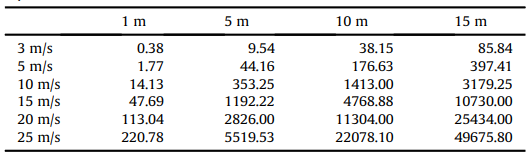
\includegraphics[width=\linewidth]{marswind}
	\caption{Wind power (W) as a function of velocities and rotor diameters on Mars {[4]}}
\end{figure}

\section*{References}
\begin{small}
{[1]} Drake, Bret G. \& Watts Kevin D.. (2014). Human Exploration of Mars Design Reference Architecture 5.0, Addendum \#2. SP-2009-566-ADD2
\\
{[2]} F. Javier Martín-Torres, María-Paz Zorzano, Patricia Valentín-Serrano, Ari-Matti Harri, Maria Genzer, Osku Kemppinen, Edgard G. Rivera-Valentin, Insoo Jun, James Wray, Morten Bo Madsen, Walter Goetz, Alfred S. McEwen, Craig Hardgrove, Nilton Renno, Vincent F. Chevrier, Michael Mischna, Rafael Navarro-González, Jesús Martínez-Frías, Pamela Conrad, Tim McConnochie, Charles Cockell, Gilles Berger, Ashwin R. Vasavada, Dawn Sumner \& David Vaniman. Transient liquid water and water activity at Gale crater on Mars. Nature Geoscience volume 8, pages357–361 (2015)
\\
{[3]} Golding EW. The generation of electricity by wind power. 1st ed. London, England: E\&F. N. Spon Ltd; 1955
\\
% solar+wind potential
{[4]} Delgado-Bonal, Alfonso \& Martín-Torres, F. J. \& Vázquez-Martín, Sandra \& Zorzano, María-Paz. (2016). Solar and wind exergy potentials for Mars. Energy. 102. 550-558. 10.1016/j.energy.2016.02.110.
\\
{[5]} ] Ahmet Duran S, Dincer I, Rosen M. Thermodynamic analysis of wind energy. Int J Energy Res 2006;30:553e66.
\\
{[6]} \url{https://technology.nasa.gov/patent/LEW-TOPS-50}
\\
% Energy gen options, solar, nuclear etc
{[7]} Cooper, Chase \& Hofstetter, Wilfried \& Hoffman, Jeffrey \& Crawley, Edward. (2010). Assessment of architectural options for surface power generation and energy storage on human Mars missions. Acta Astronautica. 66. 1106-1112. 10.1016/j.actaastro.2009.09.031.
\\
{[8]} D. Rapp, Solar energy on Mars, QSS Group, Inc. in Affiliation with JPL JPL D31342-vol. 1.
\\
{[9]} J.J. Hanak, C. Fulton, A. Myatt, P. Nath, Ultralight amorphous silicon alloy photovoltaic modules for space and terrestrial applications, American Chemical Society V 3 (1986)
\\
{[10]} Geoffrey A. Landis and Thomas W. Kerslake
Glenn Research Center, Cleveland, Ohio. Phillip P. Jenkins and David A. Scheiman, Ohio Aerospace Institute, Brook Park, Ohio. Mars Solar Power NASA/TM—2004-213367
\\
{[11]} Kenneth A. Burke, Fuel cells for space science applications, NASA/
TM—2003-212730, 2003.
\\
% Kilopower
{[12]} Gibson, Marc \& Oleson, Steven \& Poston, David \& Mcclure, Patrick. (2017). NASA's Kilopower reactor development and the path to higher power missions. 1-14. 10.1109/AERO.2017.7943946.
\\
{[13]} Mars Architecture Steering Group
NASA Headquarters Bret G. Drake, editor
NASA Johnson Space Center, Houston, Texas , NASA HEM 2009 \url{https://www.nasa.gov/pdf/373665main_NASA-SP-2009-566.pdf}
\\
% solar vs fission
{[14]} Gibson, Marc; Oleson, Steven; Poston, David; McClure, Patrick. "NASA's Kilopower Reactor Development and the Path to Higher Power Missions". NASA. Retrieved March 25, 2018
\\
{[15]} McClure, Patrick Ray (March 6, 2017). "Space Nuclear Reactor Development". Nuclear Engineering Capability Review. LA-UR-17-21904: 16. Retrieved May 16, 2018.
\\
\end{small}

\nocite{*}
\bibliography{ref}
\bibliographystyle{style}
\end{document}
